\section{Model Introduction}

Reinforcement Learning is a new branch and paradigm in the Machine Learning field. But different than the classical Supervised Learning, in RL there is no supervisor, only a reward signal. In this sense, we have an agent which interacts with the environment and receives instant rewards. Therefore, in RL, we can say that the agent's actions affect the subsequent data it receives, and that time really matters, since this data is sequential non i.i.d, and moreover, the total feedback, given by the sum of all rewards, is delayed, not instantaneous \cite{Sutton1998}. All these features make RL a quite unique research field, and it can also finds a wide range of applications, from playing board games to machines control.

The basic model for a RL approach makes use of a discrete state space for representing the agent's state $S_t$, its actions $A_t$ and its full or partial environment observations $O_t$. Thus, at each timestep $t$, the agent receives an observation $O_t$, takes an action $A_t$ and ends up in the next state $S_{t+1}$, receiving an scalar reward $R_{t+1}$. Therefore, the agent's final goal is to maximize the total future reward it gets. Figure \ref{fig:RL_basic_model} illustrates this dynamics representation.

\begin{figure}[H]
    \centering
    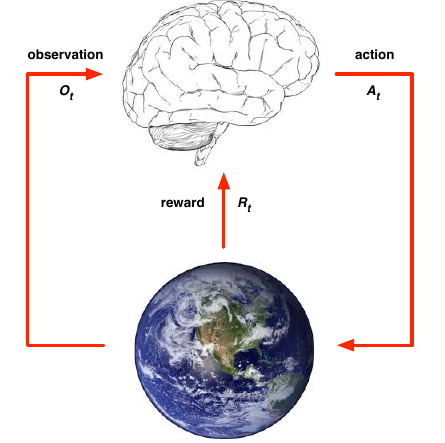
\includegraphics[width=0.4\textwidth]{Chapter2/RL_basic_model.png} 
    \caption{Agent interacting with environment.}
    \label{fig:RL_basic_model}
\end{figure}


\section{Markov Decision Processes}

A classic formal description of an environment for reinforcement learning makes use of Markov decision processes, which inherits the Markov Property from the well known Markov chains. The Markov property establish that the state of the agent captures all the relevant information from the history, in other words, the probability update function only depends of the immediate previous state, as described in \ref{eq:markov_basic}.

\begin{equation}
P(S_{t+1} | S_t) = P(S_{t+1} \mid S_1, ..., S_t)
\label{eq:markov_basic}
\end{equation}

Markov decision processes, however, has a more complete definition, it is a Markov process with rewards and actions. Basically, can be represented as a tuple $<\textbf{S}, \textbf{A}, P, R, \gamma>$, with each component defined as follows:
\begin{itemize}
\item
	$\textbf{S}$ is a finite set of states the agent can assume in the environment.
\item
	$\textbf{A}$ is a finite set of actions the agent can take.
\item
	$P$ is a state transition probability function, represented as $P_{ss'}^a = \mathbb{P}[S_{t+1}=s' \mid S_t = s, A_t = a]$
\item
	$R$ is a reward function, given by $R_s^a = \mathbb{E}[R_{t+1} \mid S_t = s, A_t = a]$
\item
	$\gamma$ is a discount factor, such that $\gamma \in [0,1]$, used to compute the cumulative total reward.
	
\end{itemize}

Besides this basic tuple representation, there are four more concepts very used in the RL literature that we must present.

\begin{itemize}
\item
	The \textbf{return} $G_T$ is the total discounted reward from time-step t, given by:
	\begin{equation}
	G_t = R_{t+1} + \gamma R_{t+2} + ... = \sum_{k=0}^{\infty}{\gamma^k R_{t+k+1}}
	\end{equation}
	Notice that by introducing the discount factor $\gamma$, it is possible to set the agent preference between short-term and long-term rewards.

	The \textbf{policy} $\pi(a \mid s)$ is a probability distribution function over actions given states, defined by:
	\begin{equation}
	\pi(a \mid s) = \mathbb{P}[A_t=a | S_t=s]
	\end{equation}
	The policy fully defines the behavior of the an agent, and can also be deterministic.
\item
	The \textbf{state-value function} $v_{\pi}(s)$ is the expected return starting from state $s$ and then following a policy $\pi$.
	\begin{equation}
	v_{\pi}(s) = \mathbb{E}_{\pi}[G_t \mid S_t = s]
	\label{eq:state_value_function_definition}
	\end{equation}
	In other words, it can be seen as a measure of how good the current agent's state is.
\item
	The \textbf{action-value function} $q_{\pi}(s,a)$ is the expected return starting from state $s$, taking action $a$, and then following policy $\pi$
	\begin{equation}
	q_{\pi}(s,a) = \mathbb{E}_{\pi}(G_t \mid S_t = s, A_t = a)
	\label{eq:action_value_function_definition}
	\end{equation}
	It can also be understood as a measure of how good it is to take a given action at the agent's current state.
\end{itemize}

\subsection{Optimality in Reinforcement Learning}

The ultimate goal of RL is finding an optimal behavior that maximizes the total expected return given by $\mathbb{E}_{R_i,S_i \sim E, A_i \sim \pi}[G_i]$. Before starting presenting the methods for achieving this goal, we must define what is optimality for value functions and policies.

\subsubsection{Optimal Value Function}

A value function is optimal if it is the maximum over all policies for all states (or state-action pairs).
\begin{itemize}
\item
	Optimal State-value function: $v_*(s) = \underset{\pi}{\textrm{max }} v_\pi(s)$
\item
	Optimal Action-value function: $q_*(s, a) = \underset{\pi}{\textrm{max }} q_\pi(s, a)$.
\end{itemize}

The optimal value functions specify the best possible performance in the MDP, which is only "solved" when we know the optimal value functions.

\subsubsection{Optimal Policy}

First, we must define a partial ordering over policies, given in equation \ref{eq:policy_ordering}.

\begin{equation}
\pi \geq \pi' \text{ if } v_{\pi}(s) \geq v_{\pi'}(s), \forall s
\label{eq:policy_ordering}
\end{equation}

The optimal policy $\pi_*$ is then defined as the best among all the others policies $\pi$, such that $\pi_* \geq \pi, \forall \pi$. Moreover, the following theorem introduces three fundamental properties about optimal policies.

\begin{itemize}
\item
There exists an optimal policy $\pi_*$ that is better than or equal to all other policies, $\pi_* \geq \pi, \forall \pi$.
\item
All optimal policies achieve the optimal value function, $v_{\pi_*}(s) = v_*(s)$.
\item
All optimal policies achieve the optimal action-value function, $q_{\pi_*}(s,a) = q_*(s,a)$.
\end{itemize}

Furthermore, a deterministic optimal policy always exists, and can be easily defined from the optimal action-value function, as described in equation \ref{eq:policy_from_greedy}.

\begin{equation}
 \pi_*(a | s) = 
\begin{cases}
    1,& \text{if } a = \underset{a'}{\textrm{argmax }} q_*(s,a')\\
    0,& \text{otherwise}
\end{cases}
\label{eq:policy_from_greedy}
\end{equation}

\section{RL Algorithms}

In order to base our future approaches in the main task, we must start presenting the classical reinforcement learning algorithms in the literature and, first of all, categorizing its different natures. The following subsections will be responsible for that.

\subsection{Categorizing RL}

RL algorithms can be classified into several types related to their problems and solutions approaches.

%RL algorithms can be classified into model free or model based, prediction or control, and value based, policy based or actor critic.

Model based algorithms are used when the model of the environment is known, and therefore, the agent can performs computations without external interaction to improves its policy. Model free algorithms, however, do not use any environment model, and it improves its policy by only interacting with the environment. These two problems conditions are respectively classified as planning and reinforcement learning problems.

Moreover, RL algorithms can also be classified as value based, policy based or actor critic. Value based algorithms are methods based on computing optimal value functions, whereas policy based algorithms make use of optimal policy search approaches. Between them, we also have an hybrid solution which combines both value function and policy search approaches. Figure \ref{fig:categorizing_RL} illustrates this classical RL categories division.

Regarding their solution nature, we also have two more classifications. Prediction algorithms are basically policy evaluation algorithms, which does not obtain any optimal policy solution, but instead, given a policy computes value functions. Control algorithms, whereas, aims to achieve an optimal policy. Besides, we still have two other classifications regarding the solution approach, that are on-policy algorithms, which learns by interacting with the world with its own policy, and off-policy algorithms, which learns an optimal policy by interacting with the world with another policy.

%Explica on e off-policy


\begin{figure}[H]
    \centering
    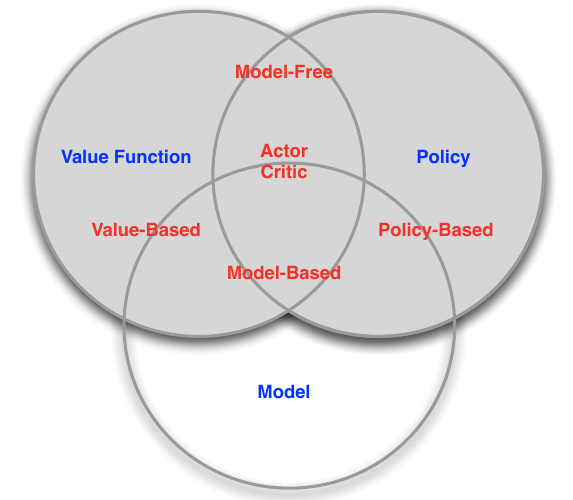
\includegraphics[width=0.5\textwidth]{Chapter2/categorizing_RL.png} 
    \caption{Classical division among RL algorithms classifications.}
    \label{fig:categorizing_RL}
\end{figure}

\subsection{Value Function Methods}

As already mentioned, value function methods employ techniques that aims to compute or estimate value functions. These algorithms are the most classic in the RL literature, and their implementation differ basically in relation to concepts like bootstrapping, bias, variance, on-policy and off-policy. In this section, we will focus on presenting only model-free algorithms, since it is from the same nature of our problem.

\subsubsection{Monte Carlo Methods}

Monte Carlo or MC methods are model-free methods that learn directly from full episodes of experience. It computes value functions through its expectation definition given in equations \ref{eq:state_value_function_definition} and \ref{eq:action_value_function_definition}. However, without a known model for the MDP, it estimates this expectation by sampling and computing the empirical mean return.

Therefore, for Monte Carlo prediction, the MC version for policy evaluation, we compute the state value $v_{\pi}(s)$ by averaging full episodic returns starting from state $s$ and running on policy $\pi$ for an arbitrarily large number of episodes in this condition.

For the control method, the main idea is to employ policy iteration, which is a basic framework for control problems which consists in an iterative solution that evaluates a given policy, by computing the value functions, and then updates this policy by acting greedy with respect to these computed value functions. Acting greedy would be choosing a deterministic policy given by equation \ref{eq:policy_from_greedy}. This loop repeats until convergence to optimal policy and optimal value functions.

In Monte Carlo model-free control, in particular, the usual approach is to use Monte-Carlo prediction to evaluate action-value functions $Q_{\pi}(s,a)$ under the policy $\pi$, then update the policy acting $\epsilon$-greedy. $\epsilon$-greedy is a simple policy update technique very similar to the greedy approach from \ref{eq:policy_from_greedy}, but it is able to ensure continual exploration. The solution for this is choosing the greedy action with $1-\epsilon$ probability, and all the others actions with the same non-zero probability. This calculation is presented in equation \ref{eq:epsilon-greedy}.

\begin{equation}
 \pi_*(a | s) = 
 \begin{cases}
    \epsilon/m + 1 - \epsilon ,& \text{if } a = \underset{a'}{\textrm{argmax }} q_*(s,a')\\
    \epsilon/m ,& \text{otherwise}
 \end{cases}
 \label{eq:epsilon-greedy}
\end{equation}

%It is possible by making that the greedy action be chosen with $1-\epsilon$ probability, whereas 

% Monte Carlo Prediction slides 6 e 7 lecture 4
% Monte Carlo Control    slides 13 ao 16 lecture 5
% Explica epsilon-greedy

\subsubsection{Temporal-Difference and Sarsa}

Temporal-Difference methods are model-free methods that are able to learn from incomplete episodes, by bootstrapping. This idea consists in updating an estimate by using another estimate obtained after taking some decision steps. In its most simple version for policy evaluation, $TD(0)$, it is possible to learn $v_{\pi}$ online while experiencing under $\pi$, by updating the estimate $V(S_t)$ toward the estimated return $R_{t+1} + \gamma V(S_{t+1})$, as given in equation \ref{eq:TD0_update}.

\begin{equation}
V(S_t) = V(S_t) + \alpha(R_{t+1} + \gamma V(S_{t+1}) - V(S_t))
\label{eq:TD0_update}
\end{equation}

For Temporal-Difference control, it is also commonly employed a policy iteration approach. We use TD to compute action-value function estimates $Q(S,A)$ given the policy $\pi$, and then use $\epsilon$-greedy to improve the policy. This method is known as SARSA, due to the process of, given a state $S$, take an action $A$, receive a reward $R$, end in a next state $S'$, and then choose another action $A'$ in order to compute the TD target. The algorithm \ref{algo:sarsa} fully describes this method.

\begin{algorithm}[H]
    \DontPrintSemicolon
    \SetAlgoLined
    Initialize $Q(s,a)$, $\forall s \in S$, $a \in A(s)$, arbitrarily, and $Q$(terminal-state,.)=0\;
    \For{episode = $1$, $M$}{
        Initiliaze $S$\;
        Choose $A$ from $S$ using policy derived from $Q$ (e.g., $\epsilon$-greedy). \;
        \For{t = $1$, ...,$T$}{
			Take action $A$, observe $R$, $S'$. \;
			Choose $A'$ from $S'$ using policy derived from $Q$ (e.g., $\epsilon$-greedy). \;
			$Q(S,A) \leftarrow Q(S,A) + \alpha(R + \gamma Q(S',A') - Q(S,A))$. \;
			$S \leftarrow S'$; $A \leftarrow A'$; \;
        }
    }
    \caption{Sarsa algorithm}
    \label{algo:sarsa}
\end{algorithm}

The SARSA algorithm is most famous for another variation, that is able to bootstrap into more future steps. The SARSA($\lambda$) method computes a different TD target $Q_t^{\lambda}$ making use of a discount weight $(1-\lambda) \lambda^{n-1}$ over n steps action-values $Q_t^{(n)}$, as shown in equation \ref{eq:sarsa_lambda}.

\begin{align}
Q_t^{\lambda} = (1 - \lambda) \sum_{i=1}^{n}{\lambda^{n-1}Q_t^{(n)}} \\
Q(S,A) = Q(S,A) + \alpha( Q_t^{\lambda} - Q(S,A))
\label{eq:sarsa_lambda}
\end{align}

The main difference between SARSA and MC control algorithms is that SARSA can learns before the end of the episode, and have low variance and some bias, whereas MC can only learn from complete episodes, and therefore has high variance and zero bias. Besides, MC has better convergence properties.

% TD lambda para prediction
% TD lambda para control com Sarsa slides 23 ao 25 lecture 5, apresentar algoritmo

\subsubsection{Q-Learning}

For off-policy learning we have some variations of the previous algorithms. The most basic ones involve importance sampling, that corrects expectations given in one distribution to another, as shown in equation \ref{eq:importance_sampling}.

\begin{equation}
\mathbb{E}_{X \sim P}[f(X)] = \mathbb{E}_{X \sim Q}\left[\frac{P(X)}{Q(X)}f(X)\right]
\label{eq:importance_sampling}
\end{equation}

The most famous off-policy algorithm though is Q-learning, that does not importance sample. Q-learning is able to improve both the behavior policy $\mu$ and the target policy $\pi$, by acting greedy w.r.t. $Q(s,a)$ for $\pi$ and acting $\epsilon$-greedy w.r.t. $Q(s,a)$ for $\mu$. The general algorithm is very similar to SARSA, with the difference that the next action is chosen using the behavior policy, and the alternative successor action is chosen using the target policy. Equation \ref{eq:qlearning_update} describes the update step for $Q(S,A)$ in Q-learning.

\begin{equation}
Q(S,A) \leftarrow Q(S,A) + \alpha (R + \gamma \underset{a'}{\textrm{max }}Q(S',a') - Q(S,A))
\label{eq:qlearning_update}
\end{equation}

\subsection{Policy Search Methods}

Policy search methods are model-free control algorithms which directly compute the optimal value function, without the use of value functions estimates, as shown in previous algorithms. In this sense, the approach consists in using a parametrized function approximation $\pi_{\theta}(a|s)$ for the policy, and the goal is to reach the desired parameters $\theta^*$ that best estimate the optimal policy, in a way that $\pi_{\theta^*}(a|s) \thickapprox \pi_*(a|s)$. Furthermore, the strategy for achieving this goal is solving an optimization problem, which comes from another perspective for the optimal policy, that is the policy that maximizes the expected total return running over several trajectories $\tau$, as defined in equations \ref{eq:tau_def} and \ref{eq:theta_max}.

\begin{align}
P_{\theta}(\tau) = P_{\theta}(s_1,a_1,...,s_T,a_T) = P(s_1)\prod_{t=1}^T{\pi_{\theta}(a_t|s_t) P(s_{t+1}|s_t,a_t)} 
\label{eq:tau_def}
\\
\theta^* = \underset{\theta}{\textrm{argmax }} J(\theta) =
\underset{\theta}{\textrm{argmax }} \mathbb{E}_{\tau \sim P_{\theta}(\tau)} \left[ \sum_t{R_t(s_t,a_t)} \right]
\label{eq:theta_max}
\end{align}

This optimization problem is solved through gradient ascent methods, and therefore we must compute the gradient of the objective function $J(\theta)$. For this propose, we can rewrite $J(\theta)$ as in \ref{eq:rewrite_objective}, and compute its gradient $\nabla_{\theta} J(\theta)$ using the manipulation described in \ref{eq:grad_with_scorefunc}, in order to work with the score function $\nabla_{\theta}\log{\pi_{\theta}(a|s)}$.

\begin{equation}
J(\theta) = \mathbb{E}_{\tau \sim P_{\theta}(\tau)} \underbrace{ \left[ \sum_t{R_t(s_t,a_t)} \right] }_{r(\tau)} = \int{\pi_{\theta}(\tau)r(\tau)d \tau}
\label{eq:rewrite_objective}
\end{equation}

\begin{equation}
\nabla_{\theta} J(\theta) = \int{\nabla_{\theta} \pi_{\theta}(\tau)r(\tau)d \tau} = 
\int{\pi_{\theta}(\tau) \nabla_{\theta} \log{\pi_{\theta}(\tau)} r(\tau)d \tau} =
\mathbb{E}_{\tau \sim \pi_{\theta}(\tau)} \left[ \nabla_{\theta} \log{\pi_{\theta}(\tau)} r(\tau) \right]
\label{eq:grad_with_scorefunc}
\end{equation}

Using the gradient $\nabla_{\theta} J(\theta)$, computed in \ref{eq:grad_with_scorefunc}, the main idea presented in \cite{REINFORCE} is making use of stochastic gradient ascent to reach $\theta^*$. The algorithm is therefore presented in \ref{algo:reinforce}.

\begin{algorithm}[H]
    \DontPrintSemicolon
    \SetAlgoLined
    Initialize $\theta$ arbitrarily\;
    \For{each episode \{ $s_1$, $a_1$, $r_2$, ..., $s_{T-1}$, $a_{T-1}$, $r_T$ \} $\sim$ $\pi_{\theta}$ }{
        \For{t = $1$, ...,$T$}{
			$\theta \leftarrow \theta + \alpha \nabla_{\theta} \log{\pi_{\theta}(s_t,a_t)} G_t$
        }
    }
    \Return{$\theta$}
    \caption{REINFORCE algorithm}
    \label{algo:reinforce}
\end{algorithm}

In comparison with value function methods, the main advantages of policy-based RL algorithms are the effectiveness in high-dimensional or continuous action spaces, the possibility to learn stochastic policies and the better convergence properties. The main disadvantages, though, are the computational inefficiency, the high variance of these methods and the usual convergence to local optimum rather than the global optimum.

% define average reward objective function
% define the goal for RL, that is theta argmax J(theta)
% derive grad J(theta) with score function and sum total reward
% present REINFORCE algo

\subsection{Actor-Critic}
% presenting the critic Qw(s,a) as a function estimate for the total return Gt

In algorithm \ref{algo:reinforce}, we used the total return $G_t$ as an unbiased sample of $Q^{\pi_{\theta}}(s_t,a_t)$, but we can also rewrite $\nabla_{\theta} J(\theta)$ as in equation \ref{eq:actor_critic_gradient}. In this sense, we could also use an action-value function approximation to derive the objective function gradient, by making use of a \textit{critic} function $Q_W(s,a) \thickapprox Q^{\pi_{\theta}}(s_t,a_t)$.

\begin{equation}
\nabla_{\theta} J(\theta) = \mathbb{E}_{\tau \sim \pi_{\theta}(\tau)} \left[ \nabla_{\theta} \log{\pi_{\theta}(\tau)} Q^{\pi_{\theta}}(s_t,a_t) \right]
\label{eq:actor_critic_gradient}
\end{equation}

Therefore, Actor-Critic methods maintain two sets of parameters to be updated toward optimum policy and action-value functions: the parameters $W$ for the \textit{critic} action-value estimate $Q_W(s,a)$, and the parameters $\theta$ for the \textit{actor} policy estimate $\pi_{\theta^*}(a|s)$.

